\documentclass[11pt]{article}
\usepackage[margin=0.7in]{geometry}
\usepackage{multirow}
\usepackage {graphicx}
\usepackage{tocloft}
\renewcommand{\cftsecleader}{\cftdotfill{\cftdotsep}}
\usepackage[utf8x]{inputenc} % указать кодировку русского текста
\usepackage[russian]{babel} % указать, что язык текста - русский
\usepackage{fancyhdr}
\pagestyle{fancy}
\graphicspath{{pictures/}}
\DeclareGraphicsExtensions{.pdf,.png,.jpg}
\begin{document}
\begin{titlepage}
\begin{center}
\large\textbf{Московский Физико-Технический Институт}\\
\large\textbf{(государственный университет)}\\
\hfill \break
\hfill \break
\hfill \break
\hfill \break
\hfill \break
\hfill \break
\hfill \break
\hfill \break
\hfill \break
\hfill \break
\hfill \break
\hfill \break
\hfill \break
\hfill \break
\hfill \break
\hfill \break
\hfill \break
\hfill \break

\huge\textbf{ Термоэлектронный диод}\\
\LARGE\textbf{Лабораторная работа по курсу вакуумная электроника}\\
\hfill \break
\hfill \break
\end{center}
\begin{flushright}
\large Выполнила студентка группы Б04-004 Шлапак Мария\\
\end{flushright}
\hfill \break
\hfill \break
\hfill \break
\hfill \break
\hfill \break
\hfill \break
\hfill \break
\hfill \break
\hfill \break
\hfill \break
\hfill \break
\hfill \break
\hfill \break
\hfill \break
\hfill \break
\hfill \break
\begin{center}
\large Факультет электроники, фотоники и молекулярной физики, 2021\\
\end{center}
\end{titlepage}
\fancyhead[L] {Термоэлектронный диод}
\tableofcontents
\newpage
\section{Цель работы}
Практическое изучение явления термоэлектронной эмиссии и процессов токопрохождения в вакууме, изготовление вакуумного диода и исследование некоторых его характеристик, проверка справедливости законов Ричардсона-Дешмана и Чайлда-Ленгмюра.\\
\section{Экспериментальная установка}
\begin{figure}[h]
    \centering
    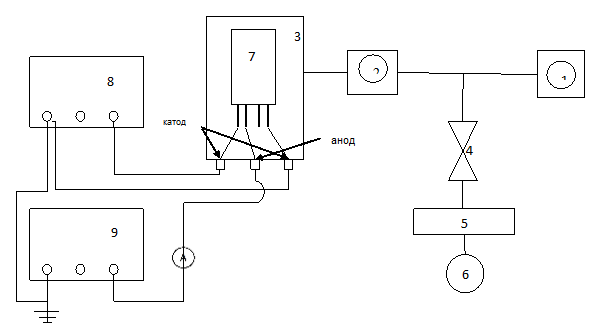
\includegraphics[width=13cm]{setup.png}
    \caption{Схема лабораторной установки}
    \label{fig:vac}
\end{figure}
\begin{enumerate}
    \item Форвакуумный насос
\item Турбомолекулярный насос
\item Вакуумная камера
\item Клапан с электрическим управлением
\item Измерительная насадка
\item Фильтр входящего воздуха
\item Диод
\item Источник питания HY 3010E
\item Вольтметр GPR-30H100
\end{enumerate}

\section{Изготовление диода}
\subsection{Изготовление анода}
 1) Для изготовления анода используем никелевую пластину $30 \times 40$ мм. Для получения большей жесткости анода на заготовке с помощью шила проводятся канавки (ребра жесткости).\\
  2) Заготовка наматывается на оправку с захлестом $3$ мм, а края пластины завальцовываются на шве для более плотного прилегания.\\
  3) Сварка производится с шагом $3$ мм. межу точками.\\
\begin{figure}[h]
\begin{center}
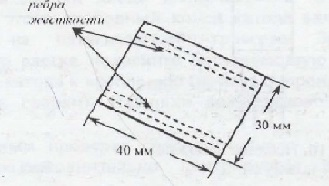
\includegraphics[width=13cm]{заготовка анода.jpg}
\end{center}
\end{figure}
\subsection{Монтаж анода на ножку}
    1) Изготавливаем траверсы из двух отрезков никелевой проволоки по $50$ мм. каждый. Проволока прокатывается между двух пластин для выравнивания и профилируется.\\
    4) Траверсы привариваются к аноду так, чтобы ось анода находилась строго между ними.\\
\begin{figure}[h]
\begin{center}
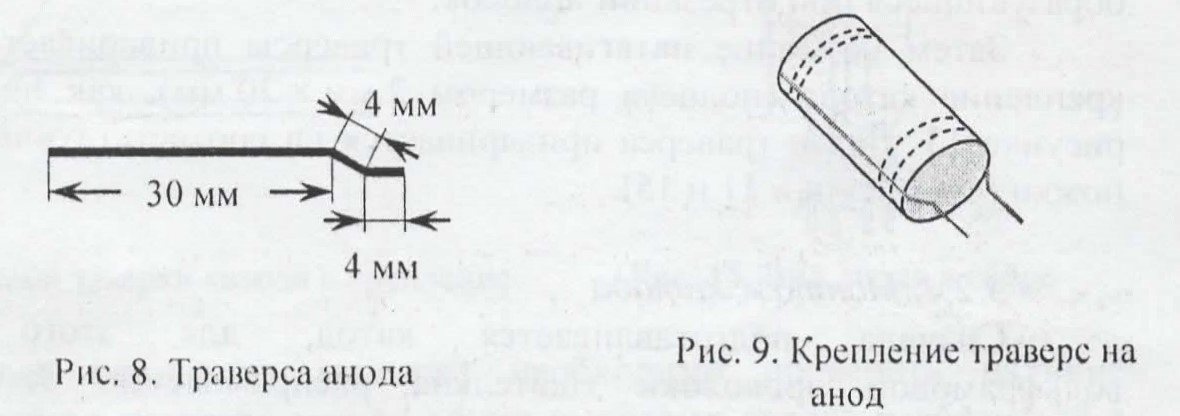
\includegraphics[width=13cm]{траверса анода.jpg}
\end{center}
\end{figure}\\
    5) Далее анод монтируется на ножку так, как показано на рисунке ниже. Предварительно надо очистить выводы ножки от окисла при помощи надфиля.\\
\begin{figure}[h]
\begin{center}
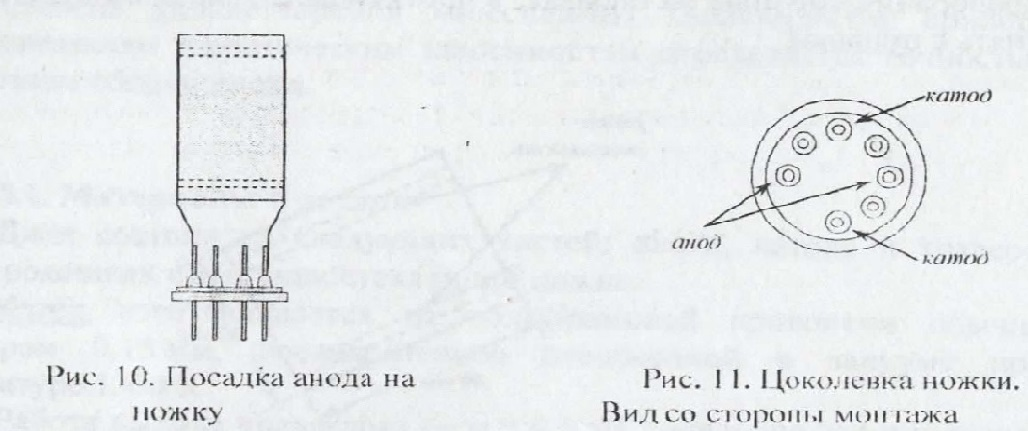
\includegraphics[width=13cm]{посадка на ножку.jpg}
\end{center}
\end{figure}
\newpage
\subsection{Подготовка крепления катода}
    1) Для изготовления катода необходимы никелевая проволока длиной $80$ мм. и две полоски из никеля размерами $2 \times 20$ мм и  $2 \times 10$ мм. Для изготовления самого катода понадобится отрезок вольфрамовой проволоки длиной $50$ мм.\\
    2) Сначала изготавливаются траверса и два крепления катода, затем на конец натягивающей траверсы приваривается первое крепление и сама траверса приваривается на соответствующий вывод ножки (см. рисунок)\\
\begin{figure}[h]
\begin{center}
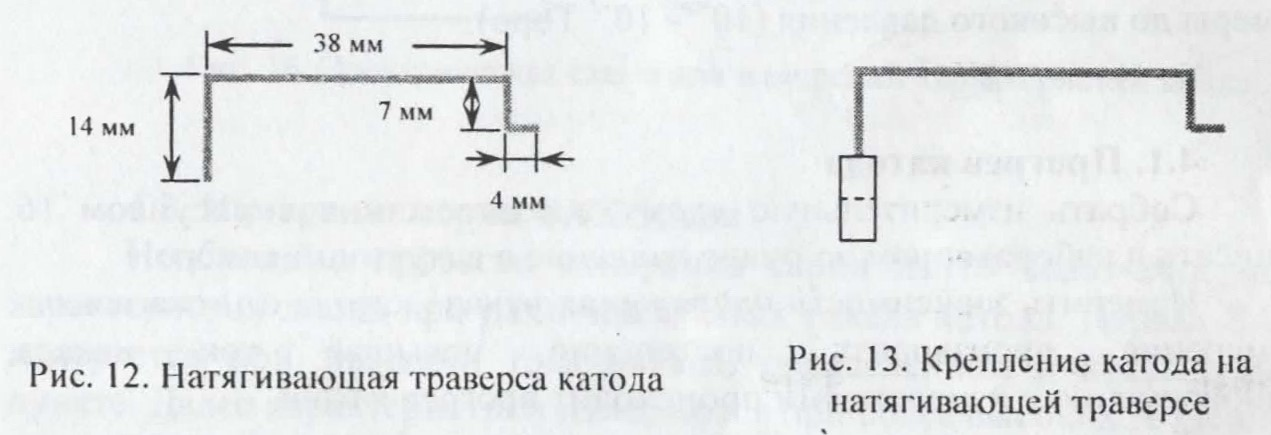
\includegraphics[width=13cm]{натягивающая траверса катода.jpg}
\end{center}
\end{figure}
\subsection{Монтаж катода}
   1) Сначала отрезок вольфрамовой проволоки распрямляется, затем катод закрепляется во втором креплении.\\
\begin{figure}[h]
\begin{center}
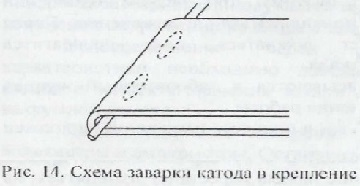
\includegraphics[width=13cm]{заварка катода.jpg}
\end{center}
\end{figure}\\
  2) Далее крепление вместе с катодом приваривается на соответствующий вывод ножки.\\
   3) Происходит натягивание и фиксация катода: для этого свободный конец катода вкладывается в согнутое крепление на натягивающей траверсе. Затем катод натягивается и его приваривают к креплению.\\
\newpage
\section{Выполнение работы}
 1)Прогреваем катод, далее снимаем зависимость тока накала от напряжения накала.Отметим также, что сопротивление вольфрамовой нити накала меняется в процессе прогрева, поэтому при резком изменении напряжения накала ток может устанавливаться не мгновенно. Полученный график представлен на рис.2\\
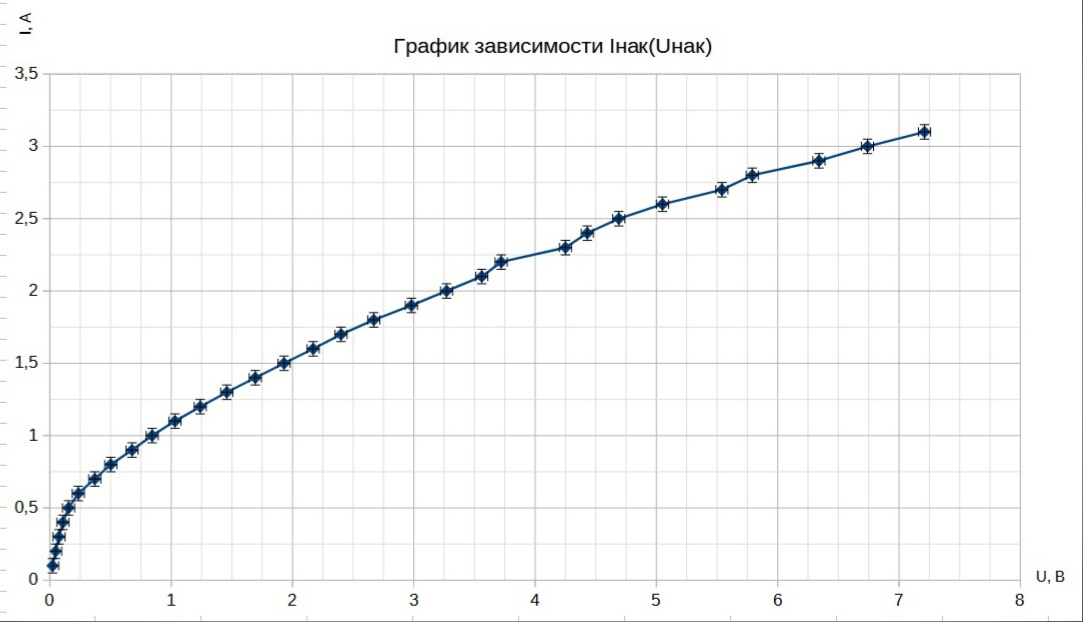
\includegraphics[width=19cm]{g1}\\
\begin{center}
Рис.2\\
\end{center}
2) Рассчитываем сопротивление диода по формуле 
\begin{center}
    $R = \frac{U}{I}$,
\end{center}
подаваемую мощность - по формуле
\begin{center}
    $P = U I$
\end{center}
3)Построим график зависимости сопротивления катода от приложенной мощности. Он изображен на рис.3\\
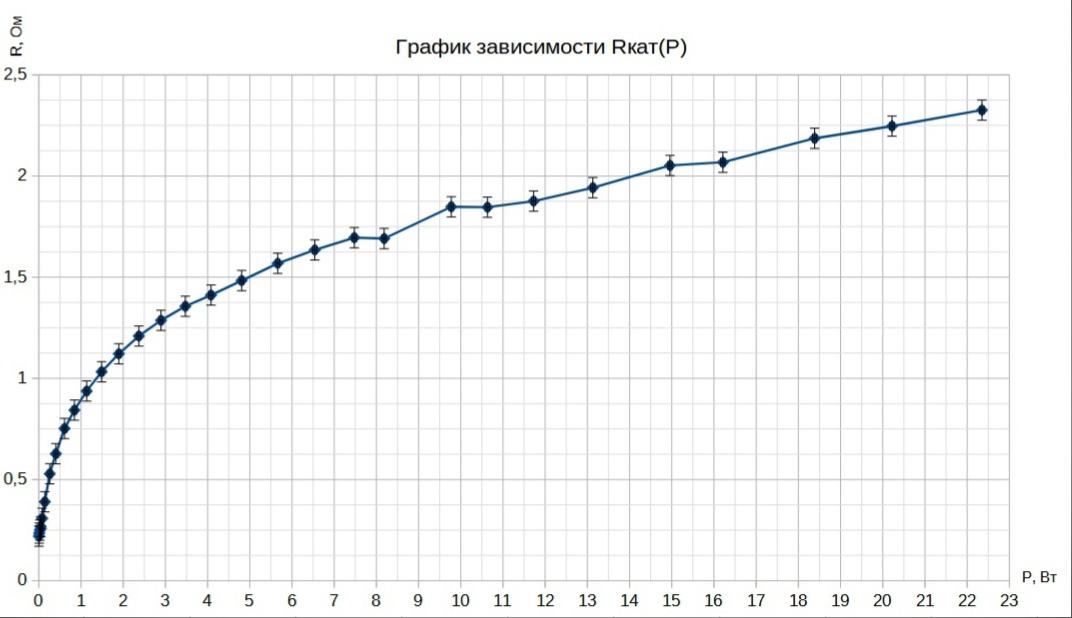
\includegraphics[width=19cm]{g2}\\
\begin{center}
Рис.3\\
\end{center}
4) Построим графики зависимости температуры катода от тока накала.  
Для графика, построенного на основании изменения сопротивления катода, температуру будем вычислять по формуле, полученной в результате преобразований:
\begin{center}
   $ \rho_T = R_0 (1 + \alpha T) $, \\
   $T = \frac{R_T - R_0}{\alpha R_0}$
\end{center}
где $\alpha = 9,29 * 10^{-3}$ - коэффициент температурной зависимости электрического сопротивления, $\rho_0$ - удельное сопротивление материала катода при $0^{\circ}$, вспомним про длину и диаметр проволоки. \\
5) Для графика, построенного на основании расчётов с использованием уравнения энергетического баланса, используем формулу 
\begin{center}
    $T_k = (\frac{P}{\varepsilon S \sigma})^{1/4}$,
\end{center}
где $S$ - площадь эмитирующей поверхности, $\varepsilon = 0.032$ - степень черноты материала катода, $\sigma = 5.67*10^{-8}$ Дж/(с*м$^2$*K$^4$). \\
На одном графике представим эти зависимости, их характеры совпадают.\\
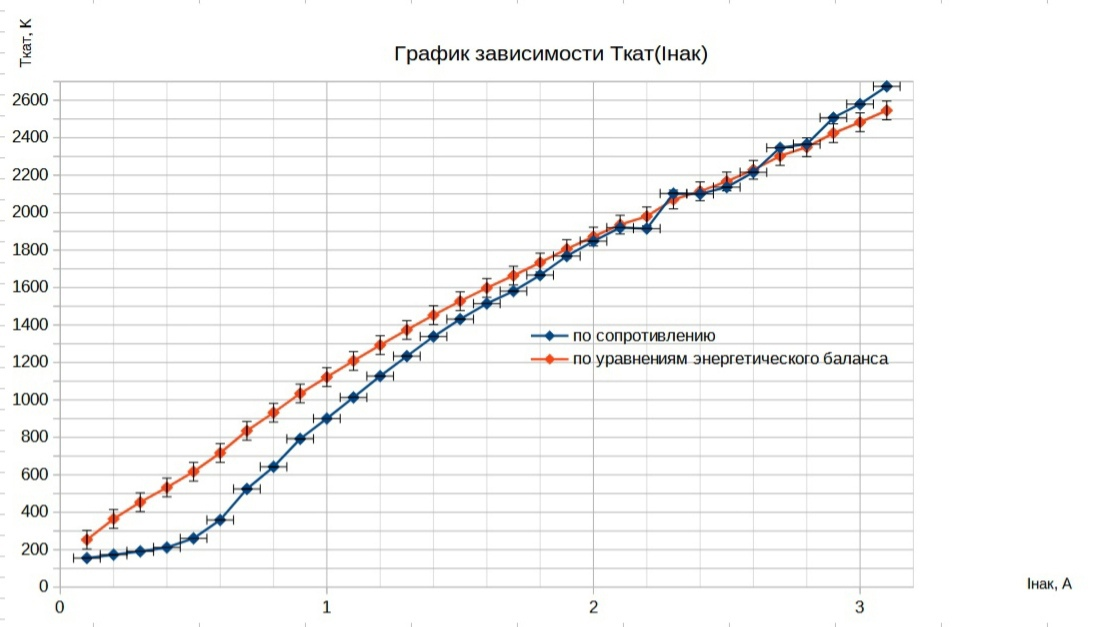
\includegraphics[width=19cm]{g3}\\
\begin{center}
Рис.4
\end{center}
6) Построим графики зависимости анодного тока от анодного напряжения пи различных значениях тока накала в координатах $lg(I_A)$ от $lg(U_A)$\\
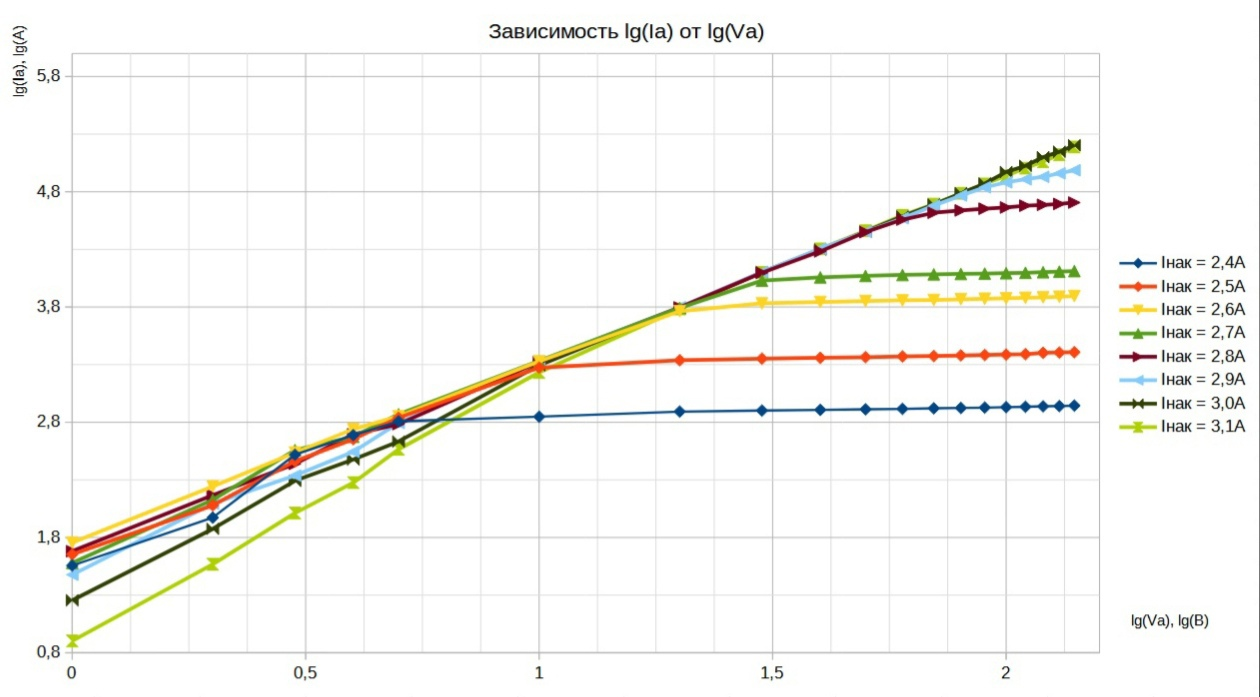
\includegraphics[width=19cm]{g4}\\
\begin{center}
Рис.5
\end{center}
7) По этим данным определим первеанс диода $g$. Зная, что $I_a = gV_A^{3/2}$ и имея зависимости $\lg(I_A) = k \lg(V_A) + b$, получим
\begin{center}
    $g = 10^{\frac{3b}{2k}}$
\end{center}
Определим первеанс по разным данным тока накала диода и сравним значения с расчётным, вычисляющимся по формуле:\\
\begin{center}
    $g = 2.33*10^{-6} \frac{S_c}{R_a ^2} = 3.4485*10^{-3}$,
\end{center}
где $S_c$ - площадь поверхности катода, $R_a$ - радиус анода. \\
Также вычислим отношение заряда электрона к его массе по формуле
\begin{center}
   $e/m = \frac{81}{8}(g\frac{R_a}{L_a})^2$
\end{center}
Наконец, эффективность катода вычислим по формуле
\begin{center}
    $\eta = \frac{I}{P}$
\end{center}
Все полученные данные запишем в таблицу:\\
    \begin{tabular}{ |p{1cm}|p{1cm}|p{1cm}|p{2cm}|p{2cm}|p{2cm}|p{2cm}|}
 \hline
 $I$, А & $U$, B & k & b & g & e/m & $\eta$, \% \\
 \hline
2.4 & 4.7 & 0.137 & -4,4898 & 6.944*$10^{-50}$ & -- & 21.3\\
 \hline
2.5 & 5.3 & 0.2409 & -4,0071 & 1.12*$10^{-25}$ & 3.528*$10^{-51}$ & 18.7\\
 \hline
2.6 & 5.5 & 0.3184 & -3,7983 & 1.27*$10^{-18}$ & 4.536*$10^{-37}$ & 18.0\\
 \hline
2.7 & 6.0 & 0.5798 & -3,7735 & 1.73*$10^{-10}$ & 8.41*$10^{-21}$ & 16.7\\
 \hline
2.8 & 6.3 & 0.7506 & -3,7191 & 3.69*$10^{-8}$ & 3.83*$10^{-16}$ & 15.9 \\
 \hline
2.9 & 6.6 & 1.0087 & -3,8266 & 2.04*$10^{-6}$ & 1.17*$10^{-12}$ & 15.0\\
 \hline
3.0 & 7.0 & 1.2219 & -3,9186 & 1.55*$10^{-5}$ & 6.75*$10^{-11}$ & 14.3\\
 \hline 
\end{tabular}\\
\\
8) Построим график зависимости анодного тока от тока накала при различных значениях напряжения на аноде Vа в координатах lg(Ia) от Iн.\\
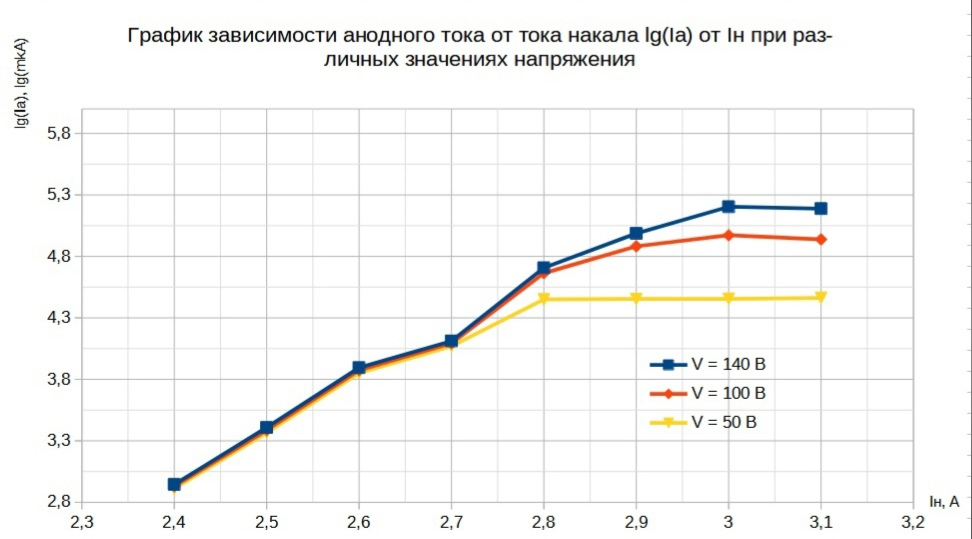
\includegraphics[width=18cm]{g5}\\
\begin{center}
Рис.6
\end{center}
\newpage

\section{Вывод}

В данной лабораторной работе по термоэлектронному диоду:
\begin{enumerate}
    \item Был изготовлен диод посредством электроконтактной сварки
    \item Были изучены следующие характеристики диода: вольт-амперная характеристика, первеанс и его эффективность
    \item Были проверены закономерности ВАХ диода: при больших токах накала - справедливо уравнение Чайлда-Ленгмюра, а при насыщении – уравнение Ричардсона-Дэшмана
    \item Была рассчитана температура катода, исходя из двух разных позиций: с точки зрения сопротивления катода, с точки зрения уравнения энергетического баланса, при помощи уравнения Ричардсона-Дэшмана построить зависимость T(I накала) не удалось, так как явной зависимости между T и I накала нет, а
численные методы решения не дали результатов, схожих с двумя предыдущими графиками.\\
\end{enumerate}
\newpage
\section{Список литературы}
\begin{enumerate}
    \item Батурин А.С., Кириченко Л.А., Коновалов Н.Д. и др. Под ред. Шешина Е.П. Эмиссионная электроника в примерах и задачах: учебное пособие / --М.:МФТИ, 2002 - 193 с. 
    \item Батурин А.С., Стариков П.А., Шешин Е.П. Термоэлектронный диод: лабораторная работа по курсу Вакуумная электроника /--М.:МФТИ, 2008 - 43 с.
\end{enumerate}

\end{document}